%https://tex.stackexchange.com/questions/37581/latex-figures-side-by-side
% put a double figure side by side

%\documentclass[12pt]{report}
%\documentclass[12pt]{extreport}
\documentclass[14pt]{extarticle}
%\documentclass{memoir}

\usepackage{graphicx}
\usepackage{setspace}
\usepackage{amsmath,amssymb}
\usepackage{IEEEtrantools}
\usepackage{cancel}
\usepackage[font=small,labelfont=bf]{caption}
\usepackage{subcaption}
\usepackage{enumitem}

\usepackage{verbatim}
%\usepackage{textcomp}
\usepackage{eurosym}


\usepackage[T1]{fontenc}
\usepackage[utf8]{inputenc}
\usepackage[italian]{babel}


%\usepackage{imakeidx}%
%\makeindex[program=xindy]%, options=-C utf8 -L portuguese]%
\usepackage{makeidx}
\makeindex




\usepackage{geometry}
 \geometry{
 a4paper,
 total={170mm,264mm},
 left=8mm,
 right=8mm,
 top=10mm,
 bottom=10mm
 }

\begin{document}

%\backmatter
%text\index{test}
%\printindex

\pagenumbering{gobble}

\begin{center}
{\bf Compito in classe di fisica}
\end{center}


\begin{enumerate}

	%Pag 117 n 19
	\item Il sistema di carrucole mostrato nella figura \ref{fig:carrucole} viene usato per sollevare una cassa di 52 kg. Osserva che una catena collega la carrucola superiore al soffitto e una seconda catena collega la carrucola inferiore alla cassa. Assumendo che le masse delle catene, delle carrucole e delle corde siaqno trascurabili, determina: 
		\begin{enumerate}
			\item la forza di richiamo $\vec{F}$ richiesta per sollevare la cassa con velocità costante;
			\item la tensione nella catena superiore;
			\item la tensione nella catena inferiore.
		\end{enumerate}
		
	%Pag 117 n 21
	\item Due blocchi sono collegati per mezzo di una corda, come in figura \ref{fig:pianoInclinato}. Il blocco che si trova sulla superficie inclinata di $30$ gradi ha una massa di $3,3$ $kg$, quello che si trova sulla superficie inclinata di $45$ gradi ha una massa di $2,6$ $kg$. Determina il modulo e il vertso dell'accelerazione dei due blocchi.
	
	%Pag 117 n 25
	\item Carlo trascina una cassa di $45$ $kg$ su un pavimento orizzontale mediante una corda inclinata di $42$ gradi. La forza con cui Carlo trascina la cassa è di $142$ $N$. 
	\begin{enumerate}
		\item Qual è la forza orizzontale che sposta la cassa in assenza di attrito con il pavimento?
		\item Qual è la forza risultante applicata alla cassa se il coefficiente di attrito dinamico tra cassa e pavimento è di $0,086$?
		\item Qual è il valore massimo del coefficiente di attrito statico tra cassa e pavimento per cui Carlo riesce a spostare la cassa?
	\end{enumerate}
\end{enumerate}




\begin{figure}[b!]
\centering
\begin{subfigure}{.5\textwidth}
  \centering
  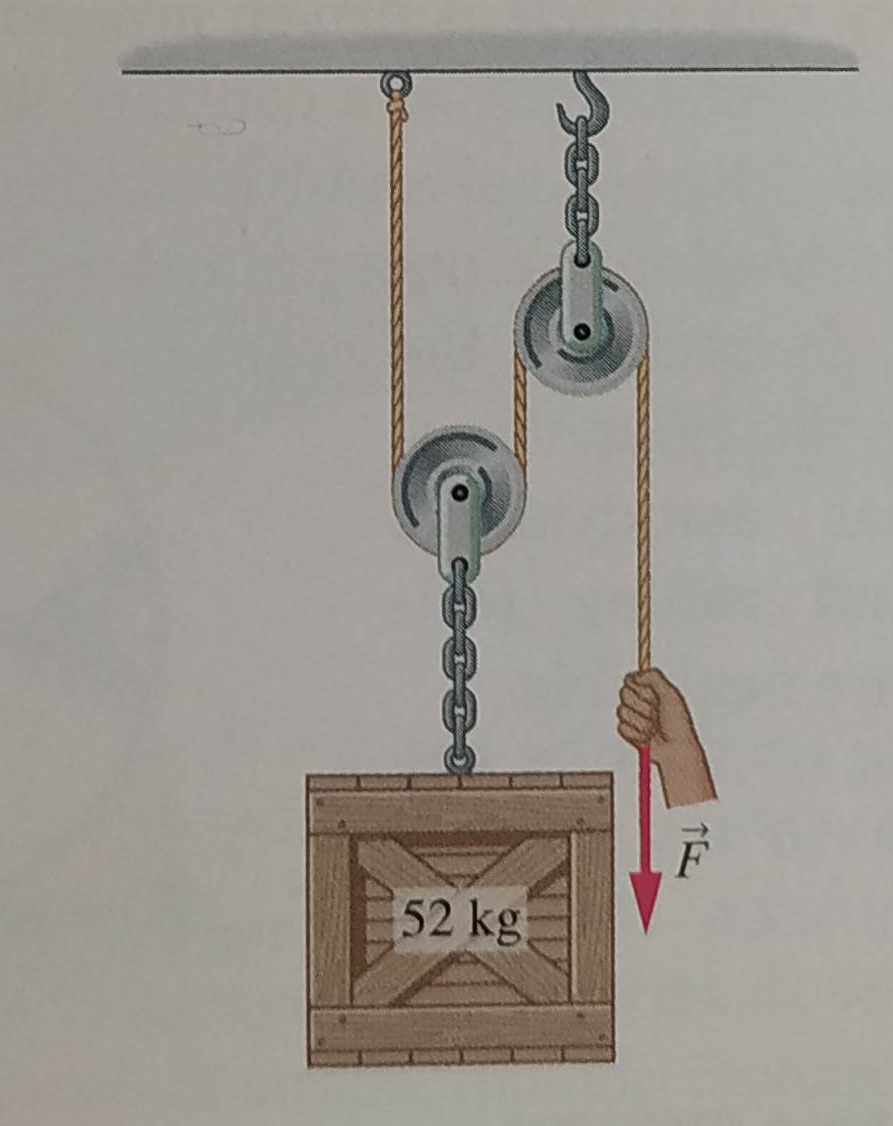
\includegraphics[width=1.8in]{pictures/problemaCarrucole.png}
  \caption{Sistema di carrucole}
  \label{fig:carrucole}
\end{subfigure}%
\begin{subfigure}{.5\textwidth}
  \centering
  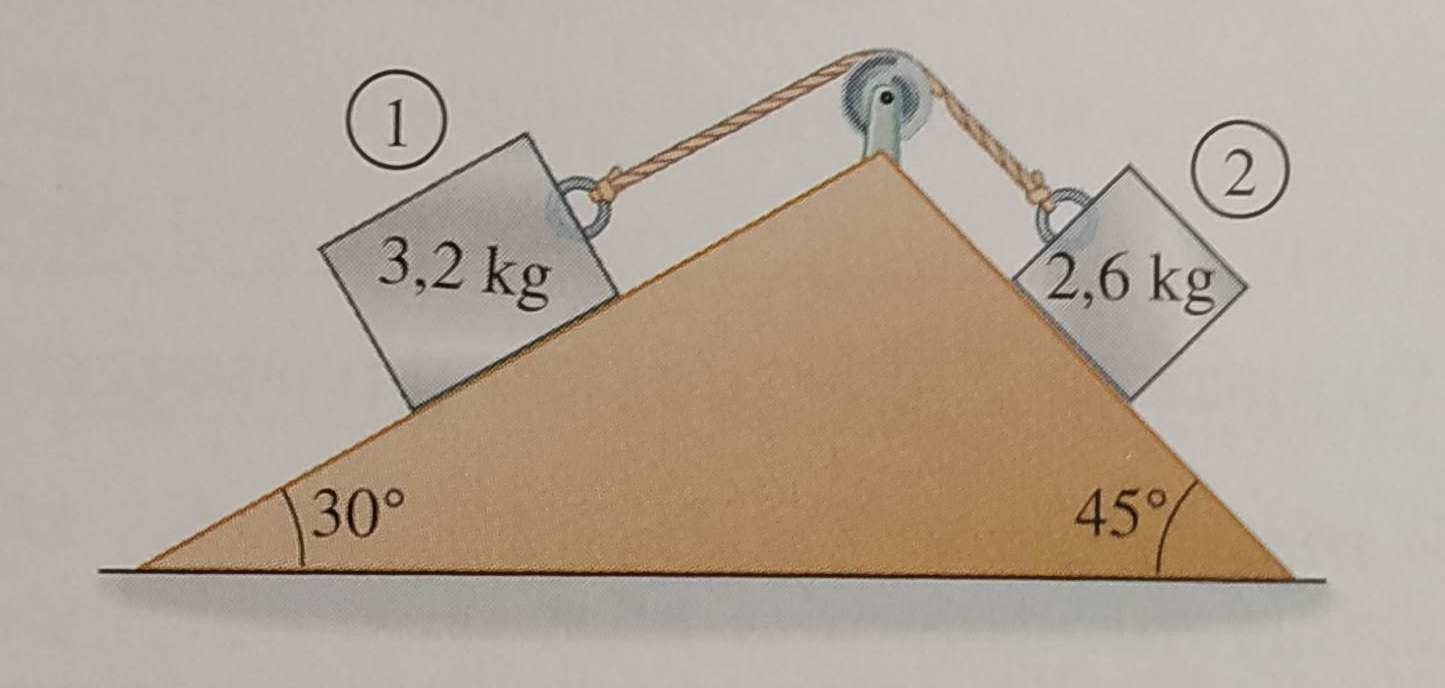
\includegraphics[width=3.8in]{pictures/problemaPianoInclinato.jpg}
  \caption{Piano inclinato}
  \label{fig:pianoInclinato}
\end{subfigure}
%\caption{A figure with two subfigures}
\label{fig:test}
\end{figure}


\end{document}